
\begin{figure}
\centering
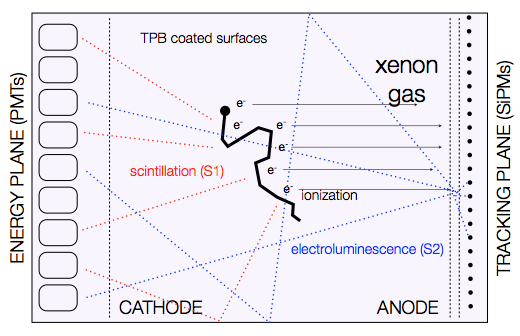
\includegraphics[width=0.9\textwidth]{img2/EL.png}
\caption{\small Principle of operation of an HPXe-EL TPC. 
} \label{fig.EL}
\end{figure}

The \emph{Neutrino Experiment with a Xenon TPC} (NEXT)\footnote{http://next.ific.uv.es/next/}  is a \bbonu\ experiment, using high-pressure (15 bar) xenon (enriched at 90\% in \XE) gas TPC with electroluminescent (EL) amplification of the ionisation signal. 

Figure \ref{fig.EL} shows the principle of operation of an HPXE-EL TPC. The detection process involves the use of the prompt scintillation light from the gas as start-of-event time, and the drift of the ionisation charge to the anode by means of an electric field ($\sim0.3$ kV/cm at 15 bar) where secondary EL scintillation is produced in the region defined by two highly transparent meshes, between which there is a field of $\sim20$ kV/cm at 15 bar. The detection of EL light provides an energy measurement using photomultipliers (PMTs) located behind the cathode (the \emph{energy plane}) as well as tracking through its detection a few mm away from production at the anode, via a dense array of silicon photomultipliers (the \emph{tracking plane}).

\subsection{NEXT prototypes}

\begin{figure}
\centering
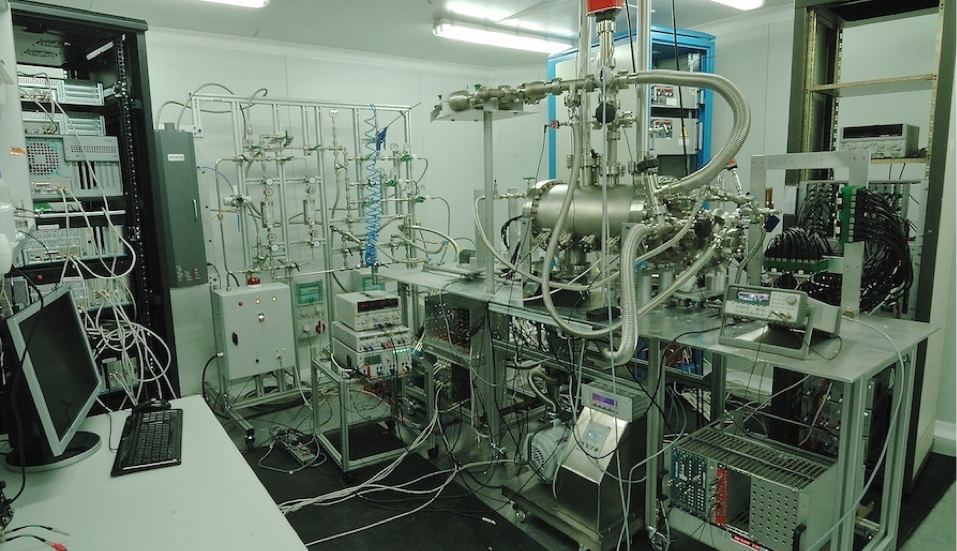
\includegraphics[width=0.9\textwidth]{img2/DemoSetup.png}
\caption{\small The NEXT-DEMO setup at IFIC (Valencia, Spain).} \label{fig.DEMO}
\end{figure}
%%%%%%%%%%
%
\begin{figure}
\centering
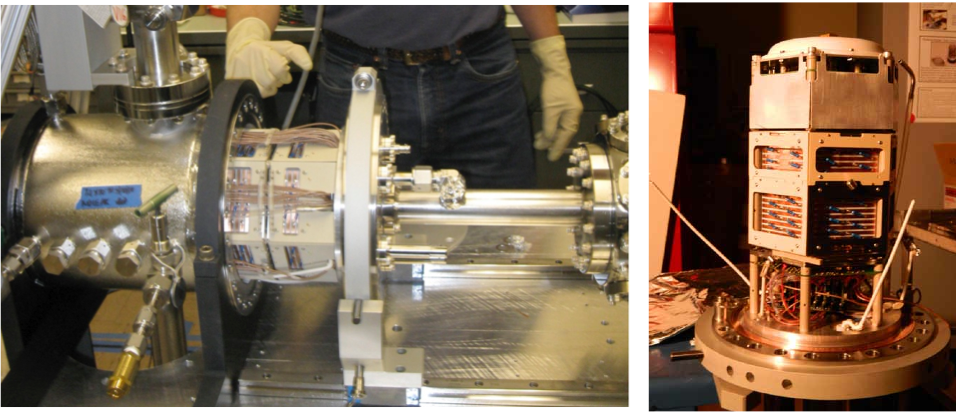
\includegraphics[width=0.9\textwidth]{img2/DBDM.png}
\caption{\small The NEXT-DBDM prototype. Top-left: the pressure vessel, in the moment in which the field cage is inserted; (b) the field cage.} \label{fig.DBDM}
\end{figure}

NEXT-DEMO, shown in figure \ref{fig.DEMO}, is as demonstrator of the HPXe-EL concept. The pressure vessel has a length of 60 cm and a diameter of 30 cm. The vessel can withstand a pressure of up to 15 bar and hosts typically 1-2 kg of xenon. NEXT-DEMO is  equipped with an energy plane made of 19 Hamamatsu R7378A PMTs and a tracking plane made of 256 Hamamatsu SiPMs. 

The detector has been operating successfully for more than four years and has demonstrated: (a) excellent operational stability, with no leaks and very few sparks; (b) good energy resolution; (c) track reconstruction with PMTs and with SiPMs coated with TPB; (d) excellent electron drift lifetime, of the order of 20 ms\cite{Alvarez:2012xda,Alvarez:2013gxa,Alvarez:2012hu}. The collaboration has just published an new article demonstrating with data the rejection power of the topological signature\cite{PFerrario:2015ina}.

The NEXT-DBDM prototype is a smaller chamber, with only 8 cm drift, but an aspect ratio (ratio diameter to length) similar to that of NEXT-100. The device has been used to perform detailed energy resolution studies, as well as studies to characterise neutrons in an \HPXE. NEXT-DBDM achieves a resolution of 1\% FWHM at 660 keV and 15 bar, which extrapolates to 0.5\% at \Qbb\cite{Alvarez:2012kua}.

\subsection{Topological signature}

%%%%%
\begin{figure}
\centering
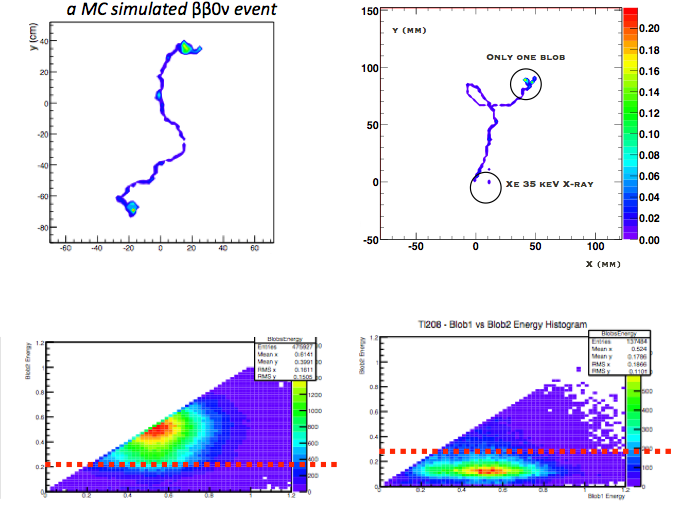
\includegraphics[width=0.9\textwidth]{img2/Topo2.png}
\caption{\small NEXT has a topological signature, not available in most \bbonu\ detectors. The top panels show the reconstruction of a Monte Carlo signal event, consisting in two electrons emanating from a common vertex (top left) and background event consisting in a single electron emitted by \BI\ or \TL\ decay (top right). The signal has two blobs of energy deposition in the track extremes, while the background has a single blob. The bottom panels show an scatter plot the energy of the blobs in the extreme of the tracks. In the case of the signal (bottom left) the energy of both blobs is high and about the same. In the case of background (top right) the energy of one blob is very small.  A simple cut requiring that the energy of both blobs is larger than a certain value (e.g, $\sim$0.2 MeV) separates effectively signal from backgrounds.}\label{fig.ETRK2}
\end{figure}
%%%%%

Double beta decay events leave a distinctive topological signature in HPXe: a continuous track with larger energy depositions (\emph{blobs}) at both ends due to the Bragg-like peaks in the 
d$E$/d$x$ of the stopping electrons (figure \ref{fig.ETRK2}, top left). In contrast, background electrons are produced by Compton or photoelectric interactions, and are characterised by a single blob and, often, by a satellite cluster corresponding to the emission of $\sim30$-keV fluorescence x-rays by xenon (figure \ref{fig.ETRK2}, top right).
Reconstruction of this topology using the tracking plane provides a powerful means of background rejection, as can be observed in the figure (see also section \ref{sec.bm}). The signal has two blobs of energy deposition in the track extremes, while the background has a single blob. The bottom panels show an scatter plot the energy of the blobs in the extreme of the tracks. In the case of the signal (bottom left) the energy of both blobs is high and about the same. In the case of background (top right) the energy of one blob is very small.  A simple cut requiring that the energy of both blobs is larger than a certain value (e.g, $\sim$0.2 MeV) separates effectively signal from backgrounds.

\subsection{Validation of the topological signature with DEMO data}

%%%%%
\begin{figure}
\centering
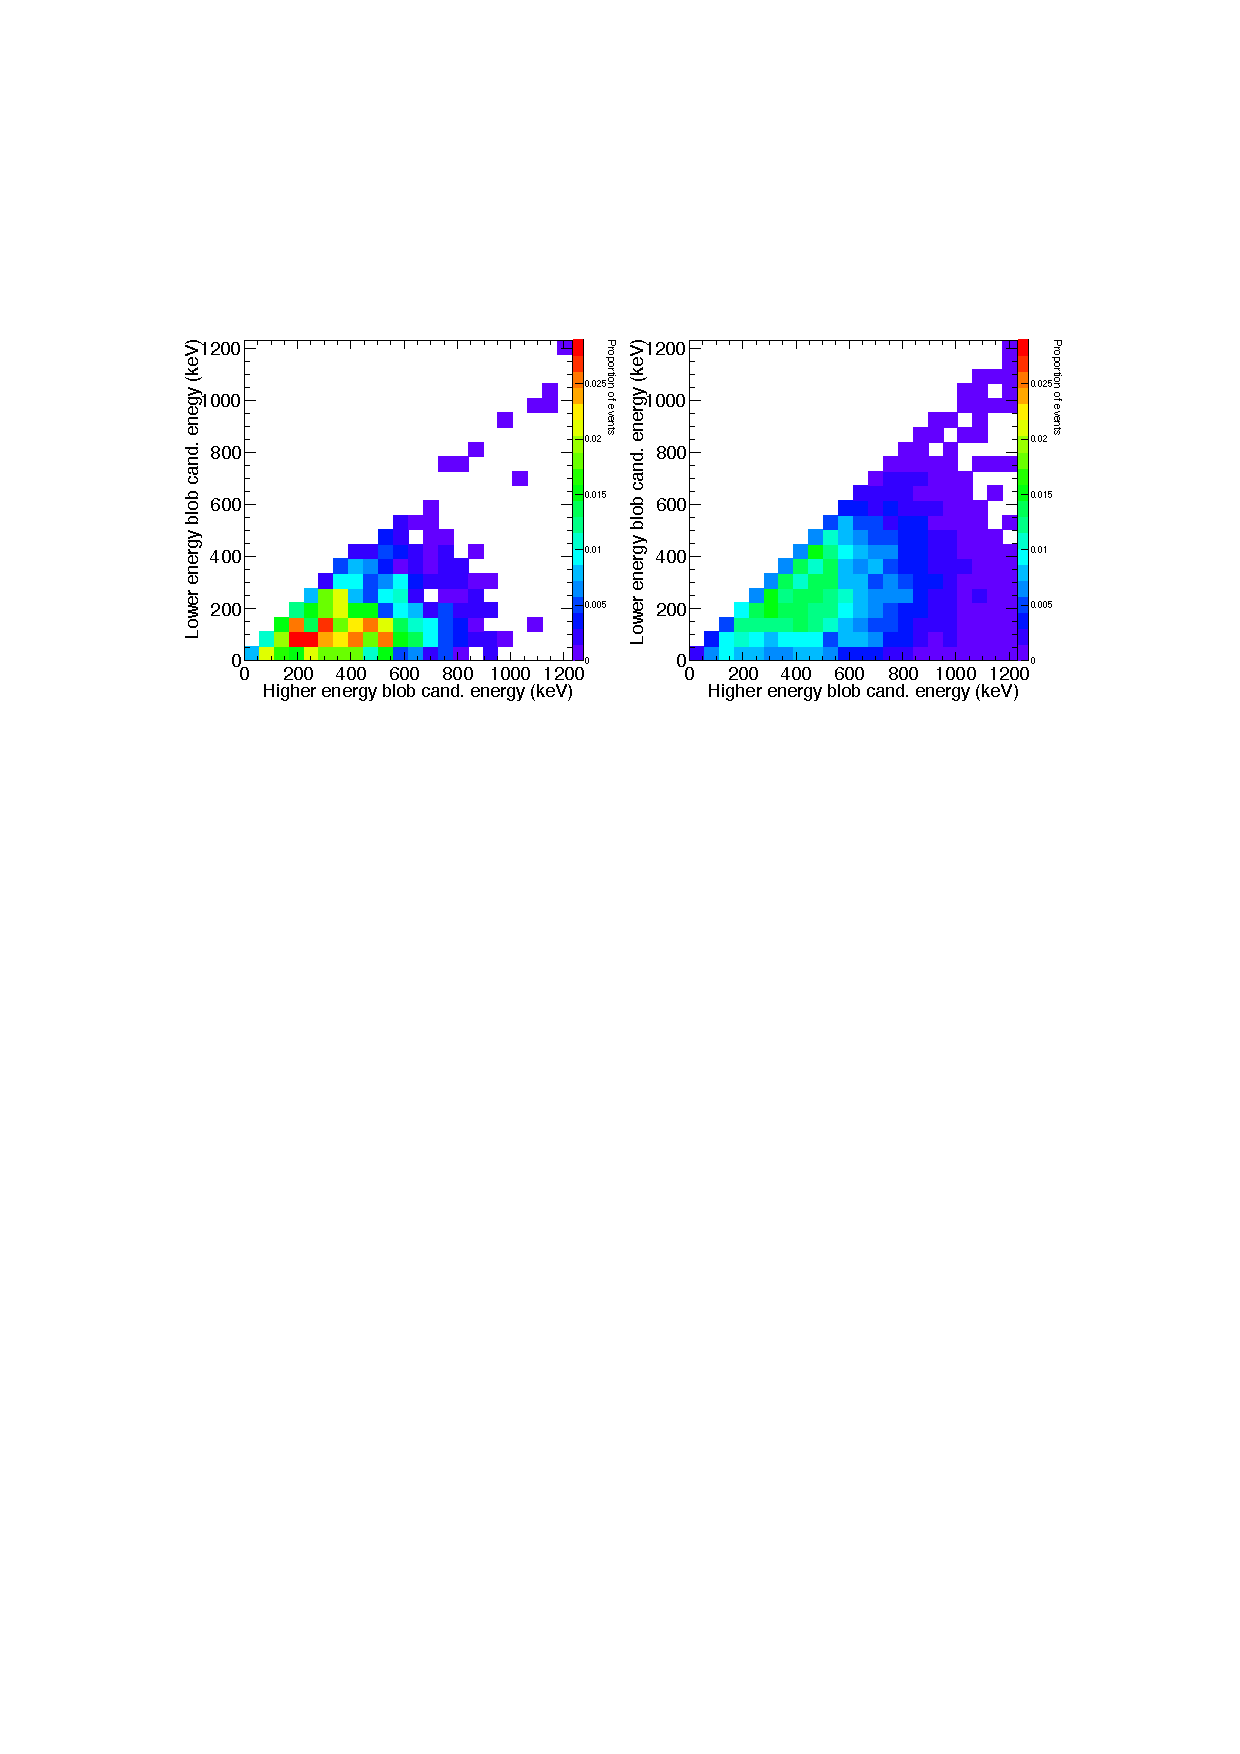
\includegraphics[width=0.9\textwidth]{img2/blobsData.pdf}
\caption{\small Energy distribution at the end-points of the tracks coming from \NA\ decay (left) and those coming from the \TL\ decay (right) for 2 cm radius blob candidates.}\label{fig.BL}
\end{figure}
%%%%% 

Figure \ref{fig.BL}, from our recently published paper \cite{PFerrario:2015ina} shows the energy distribution at the end-points of the tracks coming from \NA\ decay (left) and those coming from the \TL\ decay (right). The figure illustrates clearly that single electrons from \NA\ data are characterised by a single energetic blob, while double electrons from the double escape peak of \TL\ data show two energetic blobs. Comparison of data and Monte Carlo results using DEMO data yields an efficiency for selection \TL\ events near 70\% ($66.7 \pm 0.6$\% in data, $68.6 \pm 0.8$\% in MC). The selection efficiency for \TL\ events is smaller than for \bbonu\ events (which is around 80\%), since the tracks have less energy and thus the fraction of events with two high-energy blobs is smaller. The fraction of single electrons that pass the cut from \NA\ events is 
24\%. 

Compared to the DEMO analysis, the Monte Carlo simulation and analysis of Monte Carlo data in NEXT-100
predicts significantly improved background rejection rate of 10\% (instead of 24\%), at the same signal efficiency. A major difference which affects
these results is the relative size of the two detectors. NEXT-100 has a drift length of 1.3 m
with a circular cross section of ∼1 m and will operate at 15 bar pressure making it easily
large enough to contain electron tracks at energies similar to \Qbb\ regardless of topology
or orientation. NEXT-DEMO, on the other hand, is much smaller (the TPC has 16 cm diameter by 30 cm length). The fiducial cuts needed to contain the events tend to select tortuous tracks which do not displace as far from their origin
and are more difficult to reconstruct and more prone to blob candidate overlap. This bias,
is expected to account for the differences observed. This analysis will be repeated in 2016 with the NEW detector (see section \ref{sec.NEW}), which is only a factor two smaller than NEXT-100 (the TPC has about 0.5 m diameter and 0.5 length) and should not be affected by containment-related problems. 

\subsection{Energy resolution}

%%%%%
\begin{figure}
\centering
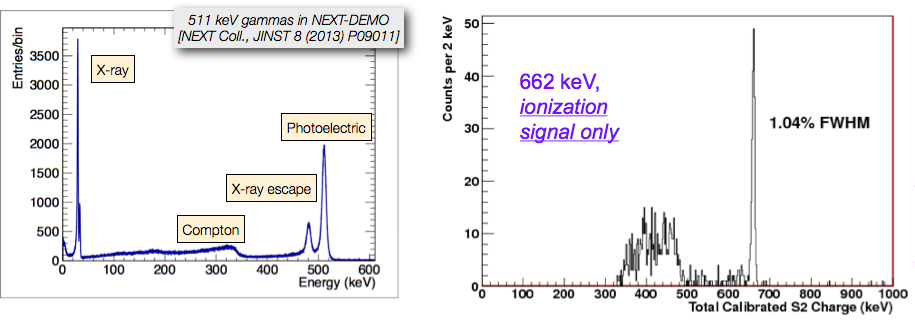
\includegraphics[width=0.9\textwidth]{img2/EResolution.png}
\caption{\small Left: the full energy spectrum measured for electrons of 511 keV in the DEMO detector. Right the spectrum near the photoelectric peak for 662 keV electrons in NEXT-DBDM. The resolution at 662 keV is 1\% FWHM (0.5\% FWHM at \Qbb). The resolution extrapolated from 511 keV is 0.7\%.}\label{fig.ERES}. 
\end{figure}
%%%%

Figure \ref{fig.ERES} shows the resolution obtained with the NEXT-DBDM apparatus. A resolution of 1\% FWHM with 
662 keV photons, has been measured, which extrapolates to 0.5\% FWHM at \Qbb. This result is not far from the expected limit obtained adding in quadrature the different factors that contribute to the resolution (Fano factor, photoelectron statistics and electronic noise). The resolution measured in NEXT-DEMO extrapolates to 0.7\% FWHM. The difference between both prototypes is due to better photoelectron statistics and aspect ratio in DBDM. The results, are, in any case, better than the target of 1\% FWHM described in the TDR. Operation with NEW (which has the same aspect ratio, roughly 1:1 than DBDM and NEXT-100) should confirm the energy resolution expected in NEXT-100. 

\subsection{NEXT-100}

\begin{figure}
\centering
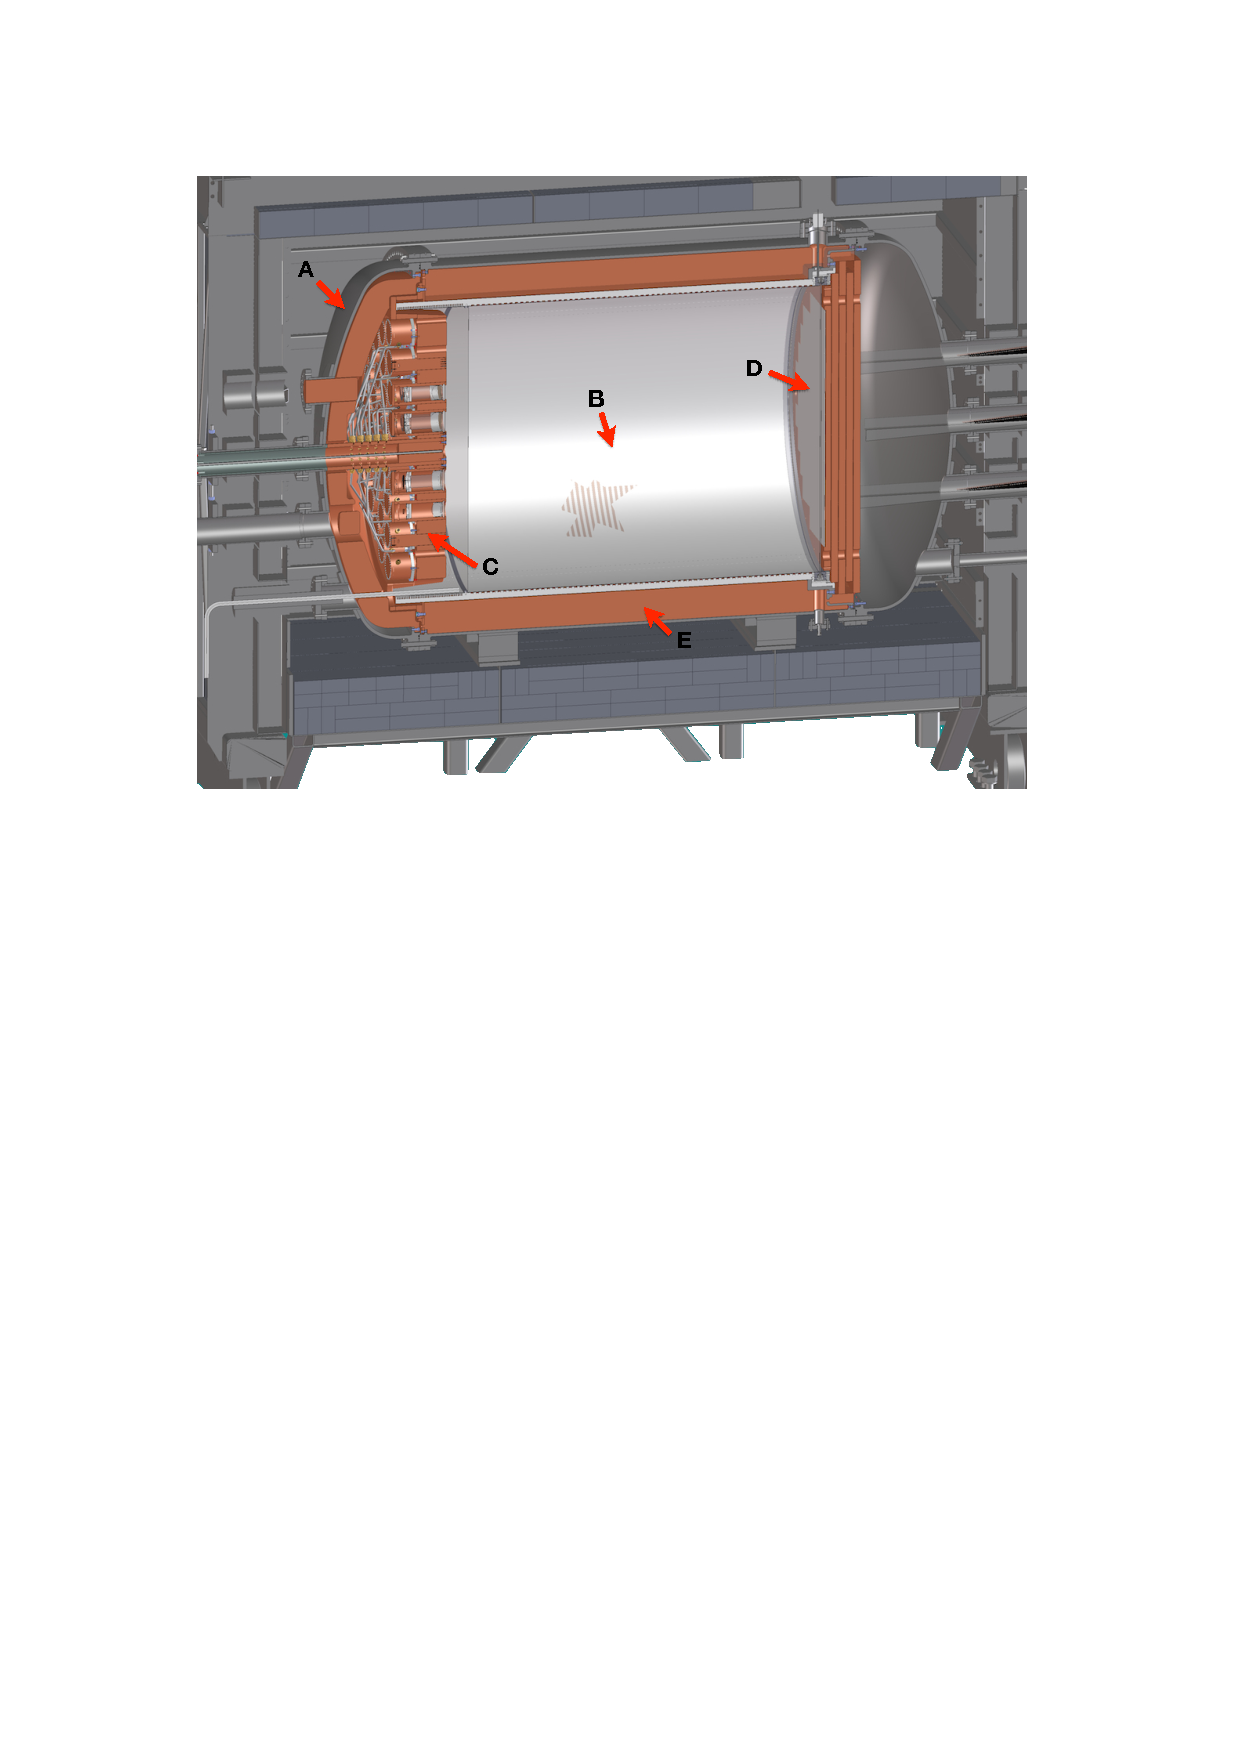
\includegraphics[width=0.9\textwidth]{img2/NEXT100.pdf}
\caption{\small Cross-section view of the NEXT-100 detector inside its lead castle shield. A stainless-steel pressure vessel (A) houses the electric-field cage (B) and the two sensor planes (energy plane, C; tracking plane, D) located at opposite ends of the chamber. The active volume is shielded from external radiation by at least 12 cm of copper (E) in all directions.
} \label{fig.NEXT100}
\end{figure}

Figure \ref{fig.NEXT100} shows a longitudinal cross-section drawing of NEXT-100 with its main components labelled. The active volume of the detector is a cylinder of approximately 1.15 m$^3$ than can hold about 100 kg of xenon gas at 15 bar. It is surrounded by an open-ended high-density polyethylene (HDPE) cylindric shell, 2.5 cm thick, 148 cm long and 107.5 cm in diameter, that provides structural stiffness and electric insulation. A series of copper rings for electric field shaping are fixed to the inner surface of the cylinder. The rings are covered by polytetrafluoroethylene (PTFE) tiles coated with tetraphenyl-butadiene (TPB) to shift the xenon VUV light to blue so as to improve the light collection efficiency. One of the ends of the HDPE cylinder is closed by a fused-silica window 1 cm thick. This window functions as the TPC anode thanks to a transparent, conductive, wavelength-shifting coating of indium tin oxide (ITO) and TPB. The two other electrodes of the TPC, EL gate and cathode, are positioned 0.5 cm and 106.5 cm away from the anode, respectively. They are built with highly transparent stainless steel wire mesh stretched over circular frames. The electrodes will be set at voltages such that a moderate electric field of 0.3--0.5 kV cm$^{−1}$~ is established in the drift region between cathode and gate, and another field of higher intensity, 2--3 kV cm$^{−1}$~ bar$^{−1}$, is created in the EL gap, between gate and anode, for the amplification of the ionization signal. The high voltage is supplied to the electrodes via radiopure, custom-made feed-throughs.

The energy plane of NEXT-100 is composed of 60 Hamamatsu R11410-10 photo-multiplier tubes located behind the cathode of the TPC and covering approximately 30\% of its area. This coverage is a compromise between the need to collect as much light as possible for a robust measurement of the energy and t$_0$, and the need to minimize the number of sensors to reduce cost, technical complexity and radioactivity. The R11410-10 is a 3-inch PMT specially developed for low-background operation. It is equipped with a synthetic silica window and a photocathode made of low temperature bialkali with quantum efficiency above 30\% for the emission wavelengths of xenon and TPB. Pressure-resistance tests run by the manufacturer showed that the R11410-10 cannot withstand pressures above 6 atmospheres. Therefore, in NEXT-100 they will be sealed into individual pressure--resistant, vacuum--tight copper enclosures closed with sapphire windows 5 mm thick. The PMTs are optically coupled to the windows using an optical gel with a refractive index intermediate between those of fused silica and sapphire. The external face of the enclosure windows is coated with TPB. The enclosures are all connected via vacuum-tight tubing conduits to a central manifold and maintained at vacuum. The PMT cables route through the conduits and the central manifold to a feedthrough in the pressure vessel nozzle.

\begin{figure}
\centering
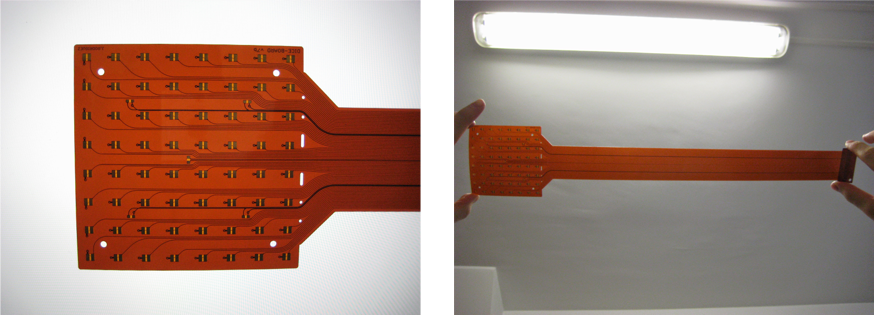
\includegraphics[width=0.9\textwidth]{img2/KDB.png}
\caption{\small The NEXT Kapton Dice Boards (KDB).} \label{fig.KDB}
\end{figure} 

The tracking function in NEXT-100 will be provided by a matrix of silicon photomultipliers (SiPMs) regularly positioned at a pitch of 1 cm and located behind the fused-silica window that closes the EL gap. The SiPMs, manufactured by SensL, have an active area of 1 mm$^2$, sensitive cells of 50 $\mu$m size, and high photon detection efficiency in the blue region (about 40\% at 440 nm). SiPMs are very cost-effective and their radioactivity is very low, given their composition (mostly silicon) and small mass. The SiPMs will be mounted on 8 × 8 flexible circuit boards made of Kapton and copper (Figure \ref{fig.KDB}). The boards have long tails that carry the signals through zigzagging slits ---so as to avoid a straight path for external gammas--- made in the copper plates that shield the active volume. The tails are connected to flat shielded cables that extract the signals from the vessel via large custom-made feed-throughs. In total, the NEXT-100 tracking plane will be composed of 7168 SiPMs distributed between 112 boards.

The sensor planes and the electric-field cage are contained within a stainless-steel pressure vessel that consists of a cylindrical central shell of 160 cm length, 136 cm inner diameter and 1 cm wall thickness, and two identical torispherical heads of 35 cm height, 136 cm inner diameter and 1 cm wall thickness. It has been fabricated with stainless steel Type 316Ti due to its low levels of natural radioactive contaminants. Designed almost entirely by the Collaboration following the ASME Pressure Vessel Code, the vessel has been built by a specialized company based in Madrid. The field cage is surrounded by a set of 12-cm thick copper bars parallel to the TPC symmetry axis, and both sensor planes are mounted to copper plates of 12 cm thickness attached to internal flanges of the vessel heads. The active volume of the detector is, therefore, shielded from external radiation by at least 12 cm of copper in all directions. The vessel sits on top of an anti-seismic pedetal and inside of a 20-cm thick lead shield made of staggered lead bricks held by a stainless-steel frame.
